\section{Introduction}

Active nematic systems are far-from-equilibrium materials characterized by broken rotational symmetry due to the local orientational order of the constituents. This asymmetry allows the energy-consuming constituents to apply anisotropic forces at a local scale leading to system-scale directional deformations. Such systems are ubiquitous in living matter, and include the actin cytoskeleton \cite{chugh2018}, microtubule and kinesin gels \cite{ndlec1997}, colonies of muscle cells \cite{duclos2014,guillamat2020}, swarms of sperm cells \cite{creppy2015},  dense bacterial suspensions \cite{qi2022, gachelin2014} and epithelial cell cultures \cite{maroudas2021,blanch2018,saw2017}. Often, these systems organize as 2D or quasi-2D material layers.
Understanding the underlying mechanism responsible for the emergence of macro- and meso-scale organizations due to micro-scale anisotropic activity is still an open challenge. Addressing this question can improve our understanding of the dynamics of living matter and potentially help us design biomimetic engineered materials \cite{fratzl2007}.

Mathematical models are widely used to explore complex systems by mapping the system of interest to mathematical equations, which can be examined analytically or numerically. Mathematical modeling of active matter in general, or the actin cytoskeleton in particular, is particularly challenging as one needs to distinguish passive dissipative and thermodynamic mechanisms from activity in a consistent manner irrespective of nonlinearity \cite{Prost:2015aa}. Formulating such models  requires a conceptual framework to guide  rational choices based on the underlying physics of the system of interest. In this context, Onsager's variational formalism provides a systematic workflow to derive fully nonlinear, multiphysics, and thermodynamically consistent mathematical models for active biological systems where inertial forces do not play a role. This framework is an extension of Rayleigh’s principle of the least energy dissipation principle \cite{Rayleigh1873} for general irreversible processes, and has been used in a number of different contexts under different names, including soft and biological matter \cite{doi2011,doi2012,arroyo2018,torres2019}.  Onsager's reciprocal relations  \cite{Onsager1931} follow naturally from this modeling formalism.


\section{Abstract statement of the Onsager's variational formalism}

We describe a dissipative system with the following key ingredients that will later serve as building blocks for the Onsager's variational formalism:
\begin{enumerate}
	\item Coarse-grained state variables $\bm{X} = \{X_1, X_2, ....X_n \}$ that identify the non-equilibrium state of the system.
	\item Free-energy potential $\mathcal{F}$ that depends on the state variables $\bm{X}$ and measures the energy available in the system to do work.
	\item Process variables $\bm{V} = \{V_1, V_2, ....V_n \}$ that describe the time evolution of the state of the system.
	\item The process operator $\mathbb{P}$, which relates the rate of change of the state variables and the process variables, i.e., $ \partial_t X_i = \mathbb{P}(\bm{X})V_i $. The process operator $\mathbb{P}$ can be trivial, i.e, $	\partial_t X_i=V_i $, or non-trivial when expressed as conservation equations, possibly involving Lie derivatives when state variables are tensor quantities.
	\item Dissipation potential $\mathcal{D}$ encoding dissipative mechanisms.
	\item Power functional $\mathcal{P}$ that encodes the external power input, e.g.~due to chemo-mechanical transduction or through boundary conditions. 
	\item A functional $\mathcal{Q}$ encoding the power done on the system by the physical constraints.
\end{enumerate}

Defining the functional form of functionals $\mathcal{F}$ and $\mathcal{D}$ determines the constitutive relations associated to passive components of the system, whereas all activity is encoded in $\mathcal{P}$.

The rate of change of the free energy potential is computed using the chain rule as
\begin{align}
	\dot{\mathcal{F}}(\bm{X};\bm{V}) =    \frac{d}{dt}\left(\mathcal{F}(\bm{X})\right)   =  \sum_{i=1}^n \partial_{X_i} \mathcal{F} \partial_t X_i 	=  \sum_{i=1}^n \partial_{X_i} \mathcal{F}\, \mathbb{P}(\bm{X})V_i. 
\end{align}
In applications, the calculations of $\dot{\mathcal{F}}(\bm{X};\bm{V})$ may imply using  Reynold's transport theorem. The dissipation potential $\mathcal{D}\left(\bm{X};\bm{V}\right)$ can be non-linear in $\bm{X}$, but is often a quadratic function of process variables $\bm{V}$. As per the thermodynamic requirements, $\mathcal{D}$ has to be non-negative, i.e, $\mathcal{D}(\bm{X},\bm{V}) \geq 0$, should be zero when the system does not evolve, i.e, $\mathcal{D}(\bm{X},0)=0$. A prototypical dissipation potential  $\mathcal{D}$ can be written as
\begin{equation}
	\mathcal{D}\left(\bm{X};\bm{V}\right) = \sum_{i=1}^{n}\sum_{j=1}^{n}V_i L_{ij}(\bm{X}) V_j,
\end{equation}
where  $L_{ij}=L_{ji}$ and $\bm{L}$ is a positive definite matrix of material coefficients according to Onsager's reciprocity relationship \cite{Onsager1931}, ensuring positivity of dissipation. The power potential $\mathcal{P}(\bm{X};\bm{V})$, in its simplest form, can be written as 
\begin{equation}
	\mathcal{P}(\bm{X};\bm{V}) = \sum_{i=1}^{n} \mathpzc{P}_{i}(\bm{X}) V_i.
\end{equation}
The constraint potential $\mathcal{Q}(\bm{X};\bm{V},\bm{\Lambda})$ is formulated as  
\begin{equation}
	\mathcal{Q}(\bm{X};\bm{V},\bm{\Lambda}) = \sum_{i=1}^{m}   \sum_{k=1}^{n} \Lambda_i C_{ik}(\bm{X})V_k ,
\end{equation}
where $C_{ij}$ is a matrix encoding constraints with $m<n$ and $\bm{\Lambda} = \{\Lambda_1, \Lambda_2, ... , \Lambda_m \}$ is a vector of Lagrange multipliers that enforces  $\bm{C}(\bm{X})\cdot \bm{V} = \bm{0}$.  By adding the aforementioned potential functions, we  form the Rayleighian as
\begin{equation}
	\mathcal{R}(\bm{X};\bm{V}) =  \dot{\mathcal{F}}(\bm{X};\bm{V}) + \mathcal{P}(\bm{X};\bm{V}) + \mathcal{D}(\bm{X};\bm{V}) .
\end{equation}
This functional captures the competition between free-energy relaxation, power input and dissipation.
Onsager’s variational principle then states that the system evolves such that
\begin{equation}
	\bm{V}  = \underset{\bm{W}}{\textup{argmin}} \, \, \mathcal{R}(\bm{X}; \bm{W}),
\end{equation}
subjected to constraints on $\bm{W}$ as 
\begin{equation}
	\sum_{j=1}^{n}	C_{ij}(\bm{X}) W_j =0.
\end{equation}
The constrained dynamics can be equivalently characterized as saddle points of the Lagrangian 
\begin{equation}
	\mathcal{L}(\bm{X};\bm{V},\bm{\Lambda}) = 	\sum_{i=1}^n \left[\partial_{X_i} \mathcal{F}\,\mathbb{P}(\bm{X}) + \mathpzc{P}_i(\bm{X}) +  \sum_{j=1}^n \left(  L_{ij}(\bm{X})V_j    -   \Lambda_j  C_{ji}(\bm{X}) \right) \right]V_i .
\end{equation}
The stationary condition $\delta_{\Lambda_i}\mathcal{L}=0$ leads to the following set of $n$ constraints
\begin{equation}
	C_{ij}(\bm{X}) V_j=0,
\end{equation}
The stationary condition $\delta_{V_i}\mathcal{L}=0$ leads to  following set of $n$ governing equations that drive the evolution of the active system of interest
\begin{equation}
\partial_{X_i} \mathcal{F}\,\mathbb{P}(\bm{X}) + \mathpzc{P}_i(\bm{X}) +  \sum_{j=1}^n \left( 2L_{ij}(\bm{X})V_j    -   \Lambda_j  C_{ji}(\bm{X}) \right)  = 0.
\end{equation}
  Towards studying active nematic systems with possibly time-dependent density in their full nonlinearity, in the following sections we develop a systematic and simple modeling framework for density-dependent active nemato-hydrodynamics using  Onsager's formalism. This theory is thermodynamically consistent ab initio, is complementary to more standard approaches based on irreversible thermodynamics for active gels \cite{Prost:2015aa,julicher2018}.


	
\section{Description of an active nematic gel} \label{sec_1}

We consider a planar thin sheet of a nematic material. We describe this system with a density field $\rho(\bm{x},t)$ and with a nematic tensor field 
\begin{equation} 
	\label{eq:nematic_tensor}
	\bm{q}(\bm{x},t) =S(\bm{x},t) \left[\bm{n}(\bm{x},t) \otimes \bm{n}(\bm{x},t) - \frac{1}{2}\bm{I}\right] ,
\end{equation}
where $\bm{I}$ is the 2D identity tensor, $\bm{n}$ is a unit vector representing the average nematic alignment and $S=\sqrt{2 q_{ab}q_{ab}}$ is the nematic order parameter, which measures the strength of the nematic alignment about $\bm{n}$. In general, $S \in [0,1]$, where $\textit{S}=0$ and $\textit{S}=1$ represent limit cases where nematic particles are isotropically distributed and perfectly aligned about $\bm{n}$, respectively. We note that $\bm{q}$ is symmetric and traceless, i.e., $\bm{q}=\bm{q}^T$ and $\text{tr}\bm{q}=0$. At any given time, the state of the system is represented by the nematic order tensor $\bm{q}$ and the density field $\rho$.

To describe how the system changes its state, we consider the macroscopic velocity field $\bm{v}$. We decompose its gradient  into a symmetric and an antisymmetric parts
\begin{align} \label{gradv}
	\nabla \bm{v}  = \bm{d} + \bm{w},
\end{align}
where 
\begin{align}
	\label{eq:rate-of-deformation}\bm{d} &= \frac{1}{2}\left[\nabla \bm{v} +\left( \nabla\bm{v}\right)^T\right],\\ 
	\label{eq:spin}\bm{w} &= \frac{1}{2}\left[\nabla \bm{v} -\left( \nabla\bm{v}\right)^T\right].
\end{align}
The tensor $\bm{d}$ characterizes the rate of deformation of a differential of volume of the material and it is usually referred to as the \textit{rate-of-deformation tensor}. This tensor plays an important role in different aspects of the theory. For instance, $\text{tr}\bm{d}=\nabla \cdot \bm{v}$ characterizes the rate of accumulation or dilution of density and its deviatoric part of $\bm{d}^{\rm dev} = \bm{d}  - \frac{1}{2}(\text{tr}\bm{d})\bm{I}$ identifies the shear rate leading to energy dissipation. The tensor $\bm{w}$ describes the local rate of rotation generated by the flow, possibly leading to rotation of the nematic alignment, and it is referred to as the \textit{spin tensor}; note that in 2D it can be represented with a single scalar $\bm{w}=w\bm{\epsilon}$, where $\bm{\epsilon}$ is the Levi-Civita tensor. The gradient of the spin is given by 
\begin{equation} 
	\bm{\zeta} = \nabla w \, .
\end{equation} 
The rate of change of $\rho$ is characterized by a conservation law of the form
\begin{equation}
	\label{eq:balance_mass}
	\dot{\rho} + \rho {\rm tr}\bm{d} = r ,
\end{equation}
where $\dot{\rho}(\bm{x},t) = \partial_t \rho(\bm{x},t) + \bm{v}(\bm{x},t)\cdot\nabla\rho(\bm{x},t)$ is the material time-derivative of $\rho$. The second term characterizes the dilution (or compaction) of $\rho$ driven by the rate of change of the differential of area characterized by the trace of $\bm{d}$, and $r$ is the rate of change of density not explained by the flow $\bm{v}$, typically resulting from a chemical reaction or a diffusive flux.  We characterize the rate of change of $\bm{q}$ with the Jaumann derivative \cite{de1993}.
\begin{equation}
	\label{eq:Jaumann}
	\widehat{\bm{q}}= \dot{\bm{q}}  + \bm{q}  \cdot \bm{w} -  \bm{w}  \cdot \bm{q},
\end{equation}
or in components as
\begin{equation} \label{jaumann_detivative_def}
	\widehat{q}_{ab} = \dot{q}_{ab}  + q_{ac} w_{cb} - w_{ac} q_{cb}.
\end{equation}
where $ \dot{q}_{ab} = \partial_t q_{ab} + v_c \nabla_c q_{ab}$ is the total time derivative of the nematic order tensor.  We note that $\widehat{\bm{q}}$ measures the rate of change of $\bm{q}$ viewed by an observer that flows and rotates with $\bm{v}$; thus, $\widehat{\bm{q}}$ is zero if $\bm{q}$ is advected and rotated by the flow without any further rearrangements of the nematic field. 

\section{Governing equations from Onsager's formalism} \label{sec:Onsager}


We derive next the governing equations of an active nematic gel at low Reynolds numbers. Let $A \subset \mathbb{R}^2$ be an open set and its boundary $\partial A$ be sufficiently smooth. The unit outward normal to $\partial A$ is denoted by $\bm{N}$.  We denote by  $\bm{t}$, $\bm{\Gamma}$ and $\bm{L}$ the boundary generalized forces power-conjugate to $\bm{v}$,  $\bm{w}$ and  $\widehat{\bm{q}}$, respectively, which we call traction, moment and microscopic moment and act on the boundaries $\partial_{N_{\bm{t}}} A $, $\partial_{N_{\bm{\Gamma}}} A $ and $\partial_{N_{\bm{L}}} A $, see Fig.~\ref{fig0}.

\begin{figure}[H]
	\centering
	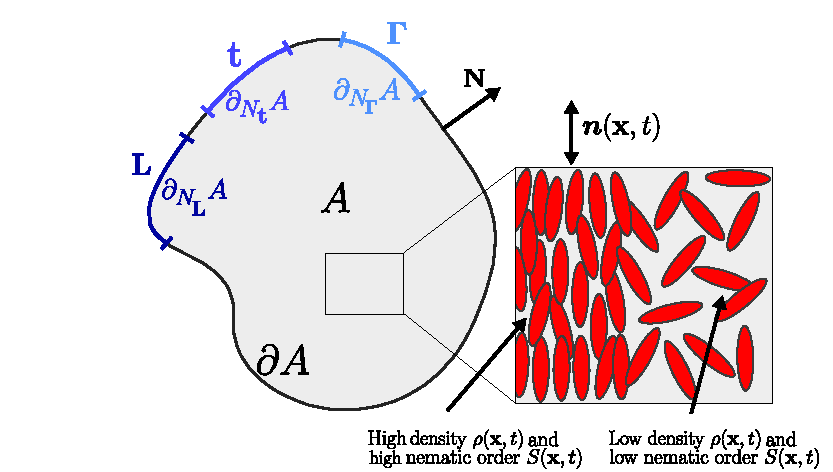
\includegraphics[width=0.75\textwidth]{chap_2_fig_1.pdf}
	\caption{\label{fig0}  \textbf{Schematic of a compressible active nematic gel}. The system occupies  a region $A$ with boundary $\partial A$ and unit outer boundary normal $\bm{N}$. Traction $\bm{t}$, moment $\bm{\Gamma}$ and microscopic moment $\bm{L}$ act on the  boundaries $\partial_{N_{\bm{t}}} A $, $\partial_{N_{\bm{\Gamma}}} A $ and $\partial_{N_{\bm{L}}} A $, respectively. The active nematic system exhibits spatiotemporal variations in density $\rho(\bm{x},t)$ and the nematic order tensor $\bm{q}(\bm{x},t)$, parametrized by the nematic order parameter $S(\bm{x},t)$ and the average molecular orientation $\bm{n}(\bm{x},t)$, Eq.~(\ref{eq:nematic_tensor}), represented with a double-headed arrow.
	}
\end{figure}
%To derive the strong form, we follow a non-linear Onsager's variational formalism. The formalism, an extension of Rayleigh’s principle of the least energy dissipation principle \cite{Rayleigh1873}, is based on the minimization of a Rayleighian functional $R = \dot{\mathcal{F}} + \mathcal{D} + \mathcal{P}$, where $\mathcal{F}$, $\mathcal{D}$ and $\mathcal{P}$ are the free energy, dissipation and power potential, repectively, possibly subject to constraints  \cite{doi2012, arroyo2018}. 

We postulate generic forms for the free-energy functional $\mathcal{F}$, dissipation functional $\mathcal{D}$ and power functional $\mathcal{P}$ as
\begin{align}
	\mathcal{F}\left[\rho,\bm{q}\right] &= \underset{A}{\int} f(\bm{q},\nabla\bm{q}) \rho dA, \label{eq:free_energy}\\
	\mathcal{D}\left[\bm{v},\widehat{\bm{q}}; \rho,\bm{q}\right] &= \underset{A}{\int} d(\bm{v},\bm{d},\bm{w},\bm{\zeta},\widehat{\bm{q}}) \rho dA,\\
	\mathcal{P}\left[\bm{v},\widehat{\bm{q}}; \rho,\bm{q}\right] &= \underset{A}{\int} p(\bm{v},\bm{d},\bm{w},\bm{\zeta},\widehat{\bm{q}}) \rho dA - \int_{\partial_{N_{\bm{t}}} A} \bm{t} \cdot \bm{v} dl -  \int_{\partial_{N_{\bm{\Gamma}}} A} \bm{\Gamma}:\bm{w} dl -  \int_{\partial_{N_{\bm{L}}} A} \bm{L}:\widehat{\bm{q}} dl,
\end{align}
where the integrands in the first three integrals are the free-energy, dissipation, and power input densities. Towards applying Onsager's variational formalism, we need to compute the rate of change of Eq.~(\ref{eq:free_energy}), for which we apply the Reynold's transport theorem 
\begin{equation}
	\begin{aligned} \label{eq:change_of_free_energy}
		\dot{\mathcal{F}} &= \underset{A}{\int} \left[\partial_tf  \rho + f \partial_t{\rho} \right] dA + \int_{\partial A} f\rho \bm{v} \cdot\bm{N} ~dl\\
		&= \underset{A}{\int} \left[\partial_tf  \rho + f \partial_t{\rho}  + \nabla\cdot\left(f\rho \bm{v}\right) \right] dA\\
		&=\underset{A}{\int} \left[\dot{f}  \rho + f \dot{\rho}  + f\rho {\rm tr}\bm{d} \right] dA.
	\end{aligned}
\end{equation}
The rate of change of $f$ can be computed as
\begin{equation}
	\begin{aligned}
		\label{eq:dotfU}  
		\dot{f} &=  \frac{\partial f}{\partial q_{ab}} \dot{q}_{ab}+ \frac{\partial f}{\partial \nabla_c q_{ab}} \dot{\nabla q}_{abc}\\
		&= \frac{\partial f}{\partial q_{ab}}\left(\widehat{q}_{ab}- q_{ad} w_{db}- q_{db} w_{da}\right) \\
		&~~~+  \frac{\partial f}{\partial \nabla_c q_{ab}}\left(\widehat{\nabla q}_{abc}-\nabla_cq_{ad} w_{db}- \nabla_cq_{db} w_{da}- \nabla_d q_{ab} w_{dc} \right), 
	\end{aligned}
\end{equation}
where $\dot{\nabla q}_{abc} = \left(\partial_t \nabla_c q_{ab} + \nabla_d \nabla_c q_{ab} v_d\right)$ and $\widehat{\nabla q}_{abc} = \dot{\nabla q}_{abc} +\nabla_cq_{ad} w_{db}+ \nabla_cq_{db} w_{da}+ \nabla_d q_{ab} w_{dc}$. We now note that $f$ must be invariant with respect to rigid body rotations, i.e.~when $d_{ab}=0$, $\widehat{q}_{ab}=0$, $\dot{f}=0$ for any $w_{ab}$. This condition can be written as
\begin{equation}
	\begin{aligned}
		0 &= \bigg[ \frac{\partial f}{\partial q_{ad}} q_{bd}  - \frac{\partial f}{\partial q_{bd}} q_{ad}  + \frac{\partial f}{\partial \nabla_c q_{ad}} \nabla_cq_{bd}-\frac{\partial f}{\partial \nabla_c q_{bd}}  \nabla_c q_{ad} \\
		&~~~+ \frac{1}{2} \left(\frac{\partial f}{\partial \nabla_a q_{cd}} \nabla_b q_{cd}-\frac{\partial f}{\partial \nabla_b q_{cd}} \nabla_a q_{cd}\right) \bigg] w_{ab},
	\end{aligned}
\end{equation}
which being valid for all spins, leads to the constraint 
\begin{equation}
	\begin{aligned}
		0 &=  \frac{\partial f}{\partial q_{ad}} q_{bd}  - \frac{\partial f}{\partial q_{bd}} q_{ad}  + \frac{\partial f}{\partial \nabla_c q_{ad}} \nabla_cq_{bd}-\frac{\partial f}{\partial \nabla_c q_{bd}}  \nabla_c q_{ad} \\
		&~~~+ \frac{1}{2} \left(\frac{\partial f}{\partial \nabla_a q_{cd}} \nabla_b q_{cd}-\frac{\partial f}{\partial \nabla_b q_{cd}} \nabla_a q_{cd}\right). 
	\end{aligned}
\end{equation}
This constraint is usually referred to as Gibbs-Duhem relation \cite{julicher2018}. Using this relation, the symmetry of $\bm{q}$ and the fact that the tensor product of a symmetric  and an antisymmetric tensor is zero, Eq.~(\ref{eq:dotfU}) reduces to
\begin{equation}
	\label{eq:dotfU2}  
	\dot{f}= \frac{\partial f}{\partial q_{ab}} \widehat{q}_{ab} +  \frac{\partial f}{\partial \nabla_c q_{ab}}\widehat{\nabla q}_{abc}.
\end{equation}
Using Eq.~(\ref{gradv}), the definition of the Levi-Civita tensor and the product rule,  the Jaumann derivative of $\nabla \bm{q}$ can be written in terms of the Jaumann derivative of $\bm{q}$ as
\begin{equation}
	\begin{aligned}
		\widehat{\nabla q}_{abc} &= \partial_t \nabla_c q_{ab} + v_d \nabla_d \nabla_c q_{ab} + \nabla_c q_{ad} w_{db} + \nabla_c q_{db} w_{da} + \nabla_d q_{ab} w_{dc}\\
		&= \nabla_c \widehat{q}_{ab} - \nabla_c v_d \nabla_d q_{ab} - q_{ad} \nabla_c w_{db} - q_{db} \nabla_c w_{da} + \nabla_d q_{ab} w_{dc}\\
		&= \nabla_c \widehat{q}_{ab} - d_{dc} \nabla_d q_{ab} - q_{ad} \nabla_c w_{db} - q_{db} \nabla_c w_{da} \\
		&= \nabla_c \widehat{q}_{ab} - d_{dc} \nabla_d q_{ab} + \left(\epsilon_{ad} q_{db} - q_{ad}  \epsilon_{db} \right) \zeta_c.
	\end{aligned}
\end{equation}
We thus can write
\begin{equation}
	\dot{f} = \frac{\partial f}{\partial q_{ab}}\widehat{q}_{ab} + \frac{\partial f}{\partial \nabla_c q_{ab}}\left[ \nabla_c \widehat{q}_{ab} - d_{dc} \nabla_d q_{ab} + \left(\epsilon_{ad} q_{db} - q_{ad}  \epsilon_{db} \right) \zeta_c\right].
\end{equation}
Plugging this expression in Eq.~(\ref{eq:change_of_free_energy}), we obtain
\begin{equation}
	\begin{aligned}
		\label{eq:dotF}
		\dot{\mathcal{F}}[\dot{\rho},\widehat{\bm{q}},\bm{d},\bm{\zeta};\rho,\bm{q}] = \int_{A} &\left\{ f \left(\frac{\dot{\rho}}{\rho}+{\rm tr} \bm{d}\right)  +\frac{\partial  f}{\partial \bm{q}} : \widehat{\bm{q}}\right.\\ 
		&\left.+ \frac{\partial  f}{\partial \nabla \bm{q}} \cdddot \, \left[\nabla \widehat{\bm{q}} - \left(\nabla \bm{q}\right)^T \cdot\bm{d} +\left(\bm{\epsilon} \cdot \bm{q} - \bm{q} \cdot \bm{\epsilon}\right)\otimes \bm{\zeta} \right]\right\} \rho dA.
	\end{aligned}
\end{equation}
For clarity of our derivation, we consider the fields $\dot{\rho}$, $\bm{d}$, $\bm{w}$ and $\bm{\zeta}$ as independent variables, and enforce the kinematic and conservation relations relating them through Lagrange multipliers. Thus, the Rayleighian has the form
\begin{align}
	\label{eq:Rayleighian}
	\mathcal{R}\left[\dot{\rho},\bm{v},\bm{d},\bm{w},\bm{\zeta},\widehat{\bm{q}};\rho,\bm{q}\right] = & \dot{\mathcal{F}}[\dot{\rho},\bm{d},\bm{\zeta},\widehat{\bm{q}};\bm{q},\rho] + 
	\mathcal{D}\left[\bm{v},\bm{d},\bm{w},\bm{\zeta},\widehat{\bm{q}}; \bm{q},\rho\right] +  \\ & \mathcal{P}\left[\bm{v},\bm{d},\bm{w},\bm{\zeta},\widehat{\bm{q}}; \bm{q},\rho\right], \nonumber
\end{align}
and the governing equations can then be obtained by minimizing it with respect to the process variables $\dot{\rho}, \bm{v},\bm{d},\bm{w},\bm{\zeta}$ and $\widehat{\bm{q}}$ and enforce kinematic and mass conservation constraints with the constraint functional
\begin{equation}
	\label{eq:constraints}
	\begin{aligned}
		\mathcal{Q}[\varrho, \bm{\sigma}^{\rm s}, \bm{\sigma}^{\rm a},\bm{m}, \dot{\rho},\bm{v},\bm{d},\bm{w},\bm{\zeta},\widehat{\bm{q}};\rho,\bm{q}] =
		& \underset{A}{\int} \varrho  \left[\dot{\rho} + \rho{\rm tr}\bm{d}- r\right] dA  + \\
		& \underset{A}{\int} \bm{\sigma}^{\rm s} :\left[\bm{d} - \frac{1}{2}\left(\nabla \bm{v} + \left(\nabla\bm{v}\right)^T\right)\right] dA + \\
		& \underset{A}{\int} \bm{\sigma}^{\rm a} :\left[\bm{w} - \frac{1}{2}\left(\nabla \bm{v} - \left(\nabla\bm{v}\right)^T\right)\right] dA + \\
		& \underset{A}{\int} \bm{m} \cdot \left[\bm{\zeta} - \nabla w\right] dA,
	\end{aligned}
\end{equation}
where $\varrho $ is the Lagrange multiplier imposing balance of mass; $\bm{\sigma}^{\rm s}$, a symmetric tensor, and $\bm{\sigma}^{\rm a}$, an antisymmetric tensor, are the Lagrange multipliers imposing the definitions of the rate-of-deformation and spin tensors; and $\bm{m}$, a vector, is the Lagrange multiplier imposing the definition of the gradient of the spin.  We thus form the  potential as 
\begin{equation}
	\label{eq:Lagrangian} 
	\begin{aligned}
		\mathcal{L}[\varrho, \bm{\sigma}^{\rm s}, \bm{\sigma}^{\rm a},\bm{m},\dot{\rho},\bm{v},\bm{d},\bm{w},\bm{\zeta},\widehat{\bm{q}};\rho,\bm{q}] =~& \mathcal{R}[\dot{\rho},\bm{v},\bm{d},\bm{w},\bm{\zeta},\widehat{\bm{q}};\rho,\bm{q}] -  \\
		&\mathcal{Q}[\varrho, \bm{\sigma}^{\rm s}, \bm{\sigma}^{\rm a},\bm{m}, \dot{\rho},\bm{v},\bm{d},\bm{w},\bm{\zeta},\widehat{\bm{q}};\rho,\bm{q}],
	\end{aligned}
\end{equation}
whose minimization with respect to the process variables leads to the governing equations. Arbitrary variations of $\widehat{\bm{q}}$ lead to
\begin{equation}
	\label{eq:var_q}
	\begin{aligned}
		0&=\underset{A}{\int} \left[ \left(\frac{\partial  f}{\partial \bm{q}} + \frac{\partial d}{\partial \widehat{\bm{q}}}+ \frac{\partial p}{\partial \widehat{\bm{q}}} \right) : \delta \widehat{\bm{q}} + \frac{\partial f}{\partial \nabla \bm{q}} \cdddot\, \nabla \delta \widehat{\bm{q}} \right] \rho dA - \int_{\partial_{N_{\bm{L}}}A} \bm{L}:\delta\widehat{\bm{q}} dl \\
		&=\underset{A}{\int} \left[\rho \left(\frac{\partial  f}{\partial \bm{q}} + \frac{\partial d}{\partial \widehat{\bm{q}}}+ \frac{\partial p}{\partial \widehat{\bm{q}}} \right) - \nabla\cdot \left(\rho \frac{\partial f}{\partial \nabla \bm{q}} \right)   \right] : \delta \widehat{\bm{q}}  dA \\
		&+ \int_{\partial_{N_{\bm{L}}}A} \left(\rho \frac{\partial f}{\partial \nabla \bm{q}} \cdot\bm{N} -\bm{L}\right):\delta\widehat{\bm{q}} dl. 
	\end{aligned}
\end{equation}
Localizing the equation above, we obtain
\begin{align}
	\label{eq:balance_q} 
	\rho \left(\frac{\partial  f}{\partial \bm{q}} +  \nonumber \frac{\partial d}{\partial \widehat{\bm{q}}} +  \frac{\partial p}{\partial \widehat{\bm{q}}}\right) - \nabla\cdot \left(\rho \frac{\partial f}{\partial \nabla \bm{q}}\right)   &= \bm{0} \qquad \text{on } A ,\\
	\rho \frac{\partial  f}{\partial \nabla \bm{q}} \cdot\bm{N} &= \bm{L} \qquad \text{on } \partial_{N_{\bm{L}}} A,
\end{align}
which represent the balance generalized forces  power-conjugate to $\widehat{\bm{q}}$. Variations with respect to $\bm{d}$ provide a definition for $\bm{\sigma}^{\rm s}$:
\begin{equation} 
	\label{eq:sym_stress}
	\sigma^{\rm s}_{ab} = -\frac{1}{2}\rho \left(\frac{\partial  f}{\partial \nabla_b q_{dc}} \nabla_a q_{dc}+ \frac{\partial  f}{\partial \nabla_a q_{dc}} \nabla_b q_{dc}\right) + \rho \frac{\partial  d}{\partial d_{ab}}+ \rho \frac{\partial  p}{\partial d_{ab}},
\end{equation}
where we have used the fact that variations with respect to $\dot{\rho}$ lead to $\varrho  = -f$. Variations with respect to $\bm{\zeta}$ lead to
\begin{equation}
	\label{eq:moment}
	m_c = 2 \rho \epsilon_{ad} \frac{\partial  f}{\partial \nabla_c q_{ab}} q_{db} + \frac{\partial  d}{\partial \zeta_c} + \frac{\partial  p}{\partial \zeta_c}.
\end{equation}
Variations with respect to $\bm{w}$ lead to
\begin{equation}
	\begin{aligned}
		0&=\underset{A}{\int} \left[-\bm{\sigma}^{\rm a} :\delta\bm{w} + \frac{1}{2} \bm{m}  \nabla \left(\bm{\epsilon}:\delta\bm{w}\right) - \bm{\omega} :\delta \bm{w} \right] dA - \int_{\partial_{N_{\bm{L}}}A} \bm{\Gamma}:\delta\bm{w} dl \\
		&=\underset{A}{\int} -\left[\bm{\sigma}^{\rm a}  + \frac{1}{2} \left(\nabla \cdot \bm{m}\right) \bm{\epsilon} +  \bm{\omega}  \right] : \delta\bm{w} dA + \int_{\partial_{N_{\bm{L}}}A} \left[\left(\bm{m}\cdot\bm{N}\right) \bm{\epsilon}- \bm{\Gamma}:\delta\bm{w}\right] dl \\
	\end{aligned}
\end{equation}  
and hence 
\begin{equation}
	\label{eq:balance_angular_momentum}
	\begin{aligned}
		\bm{\sigma}^{\rm a} + \frac{1}{2}\left(\nabla\cdot\bm{m}\right)\bm{\epsilon} +  \bm{\omega} &= \bm{0} \qquad \text{on } A,\\
		(\bm{m}\cdot\bm{N})\bm{\epsilon} &= \bm{\Gamma} \qquad \text{on } \partial_{N_{\bm{\Gamma}}} A,\\
	\end{aligned}
\end{equation}
where 
\begin{equation}
	\omega_{ab} = - \rho \left(\frac{\partial  d}{\partial w_{ab}} + \frac{\partial  p}{\partial w_{ab}}\right).
\end{equation}
Eq.~(\ref{eq:balance_angular_momentum}) represents balance of angular momentum, with $\bm{m}$ playing the role of the moment in a Cosserat theory \cite{cosserat1896theorie} and $\bm{\omega}$ the  body torques.	This equation provides a definition for $\bm{\sigma}^{\rm a}$. Finally, variations with respect to $\bm{v}$ lead to 
\begin{equation}
	\label{eq:weak_v}
	\begin{aligned}
		0 &= \underset{A}{\int} \left[\bm{\sigma}:\nabla\delta\bm{v} - \delta\bm{v}\cdot\bm{f} \right]dA - \int_{\partial_{N_{\bm{t}}} A}  \bm{t} \cdot \delta\bm{v} dl\\
		&=\underset{A}{\int} \left[-\nabla\cdot\bm{\sigma} - \bm{f} \right] \cdot \delta\bm{v}dA + \int_{\partial_{N_{\bm{t}}} A} \left(\bm{\sigma}\cdot \bm{N} -\bm{t} \right)\cdot \delta\bm{v} dl.
	\end{aligned}
\end{equation}
and hence 
\begin{equation}
	\label{eq:balance_linear_momentum}
	\begin{aligned}
		\nabla\cdot\bm{\sigma} + \bm{f} &= \bm{0} \qquad \text{on } A,\\
		\bm{\sigma}\cdot\bm{N} &= \bm{t} \qquad \text{on } \partial_{N_{\bm{t}}} A,\\
	\end{aligned}
\end{equation}
where $\bm{\sigma}=\bm{\sigma}^{\rm s} + \bm{\sigma}^{\rm a}$ and 
\begin{equation}
	\bm{f}=-\rho \left(\frac{\partial  d}{\partial \bm{v}} + \frac{\partial  p}{\partial \bm{v}}\right).
\end{equation}
Eq.~(\ref{eq:balance_linear_momentum}) represents balance of linear momentum in the 
absence of inertia; we can identify $\bm{\sigma}$ as the stress tensor, with $\bm{\sigma}^{\rm s}$ and $\bm{\sigma}^{\rm a}$  its symmetric and antisymmetric parts, and $\bm{f}$ as the body forces on the active gel.  Finally, variations with respect to $\varrho $, $\bm{\sigma}^{\rm s}$ and $\bm{\sigma}^{\rm a}$ lead to balance of mass (Eq.~(\ref{eq:balance_mass})) and the definitions of the rate-of-deformation and spin tensors, Eqs.~(\ref{eq:rate-of-deformation}) and~(\ref{eq:spin}).

\section{Model for a compressible active nematic gel} \label{sec_3}

In the previous section, we have introduced a description of an active nematic gel and derived the governing equations in terms of a rather generic free-energy,  dissipation and power potentials. Here, we make specific choices for free-energy, dissipation and power input to derive the governing equations for a density-dependent active nematic gel. 

For the free-energy density, we assume a Landau expansion
\begin{equation} 
	\label{eq:landau}
	f = \frac{1}{2}a S^2 + \frac{1}{8}b S^4 + \frac{1}{2} L \left|\nabla \bm{q}\right|^2,
\end{equation}
where $L>0$ is the Frank constant penalizing gradients of orientation and $a$ and $b$ are susceptibility parameters. For $a>0$, the susceptibility parameters penalize deviations from the isotropic state given by $S=0$. For $a<0$, the susceptibility parameters penalize deviations from anisotropic states given by $S= \sqrt{2|a|/b}$, where $b>0$. 

We consider the power density generated by the out-of-equilibrium molecular processes or activity to be of the form
\begin{align} \label{eq:pow_density_example}
	p= &  \lambda \textup{tr}\bm{d} + \lambda_{\rm aniso} \bm{q}:\bm{d}  \nonumber   -(\lambda_{\bigodot}' + \rho \lambda_{\bigodot})  \bm{q} : \widehat{\bm{q}} \\ &  =  \lambda \left(\bm{\delta} + \kappa \bm{q}\right) : \bm{d} - \rho \lambda_{\bigodot}  \bm{q} : \widehat{\bm{q}}.
\end{align}
where the first term in the first line represents the power of an isotropic active tension, the second term is the power of an anisotropic active tension along the  nematic tensor, and the third term is the power of an active generalized force conjugate to changes nematic order, with a coefficient which we expand in terms of density. We note that the constant term $\lambda_{\bigodot}'$ has a formally equivalent effect in the governing equations as the first term in Eq.~(\ref{eq:landau}), and hence can be subsumed in susceptibility parameter $a$.  For this reason we consider $\lambda_{\bigodot}'= 0$ in the second line, where  we group active tensions in a single term by defining the tension anisotropy parameter $\kappa=\lambda_{\rm aniso}/\lambda$. For $\lambda_{\bigodot}>0$, nematic activity tends to further increase alignment.

For the dissipation potential, we consider the dissipation due to shear characterized by the viscosity $\eta$, the internal dissipation due to the rate of change of nematic order characterized by the viscosity $\eta_{\text{rot}}$, the dissipation due to sliding of the nematic components with respect to the velocity gradient characterized by the coupling parameter $\beta<0$, and the friction with a substrate characterized by the friction coefficient $\gamma$
\begin{equation}
	\label{eq:diss_density_example}
	d =  \eta \left(|\bm{d}|^2 + \left(\text{tr}\bm{d}\right)^2\right) +\frac{\eta_{\text{rot}}}{2}  \left|\widehat{\bm{q}}\right|^2+ \beta  \bm{d}^{\rm dev}:\widehat{\bm{q}}  + \frac{\gamma}{2} \left|\bm{v}\right|^2.
\end{equation}
Note that for this dissipation to be positive, $2\eta \eta_{\text{rot}} - \beta^2 > 0$, see appendix~\ref{inequality}. We also note that the form of the first term in Eq.~(\ref{eq:diss_density_example}) can be motivated by assuming that the material is incompressible in three dimensions so that its three-dimensional rate of deformation tensor has an out-of-plane component $D_{33} = -{\rm tr} \bm{d}$ and the dissipation in terms of $\bm{D}$ has the form $\eta |\bm{D}|^2= \eta(|\bm{d}|^2 + \left(\text{tr}\bm{d}\right)^2)$ as for a usual Newtonian fluid \cite{salbreux2009}.

Applying the proposed density potential functionals in Eqs.~(\ref{eq:landau}-\ref{eq:diss_density_example}) to the Onsager's formalism in Section~\ref{sec:Onsager} yields the following generalized force balance equation
\begin{align}  \label{first_govern}
	\eta_{\text{rot}} \widehat{\bm{q}} + \beta \bm{d}^{\rm dev} + (2a + b S^2)  \bm{q} - L \left(\Delta \bm{q} +   \nabla\bm{q} \cdot \frac{\nabla \rho}{\rho} \right) - \rho\lambda_{\bigodot} \bm{q} = 0,
\end{align}
and balance of linear momentum
\begin{equation}
	\label{eq:balance_forces_linear}
	\nabla\cdot\bm{\sigma} = \rho \gamma \bm{v},
\end{equation}
where the stress is the sum of the symmetric stress
\begin{equation}
	\sigma^{\rm s}_{ab} = \rho \left[2\eta  (d_{ab}+d_{cc} \delta_{ab}) + \beta  \widehat{q}_{ab}  + \lambda \left(\delta_{ab} + \kappa q_{ab}\right) -L\nabla_b q_{cd} \nabla_a q_{cd}\right],
\end{equation}
and the antisymmetric stress
\begin{equation}
	\sigma^{\rm a}_{ab} = L \nabla_c \rho \left( q_{ad} \nabla_c q_{db}  - q_{bd} \nabla_c q_{da}  \right) + \rho L  \left(q_{ae}\Delta q_{be}  -q_{be}  \Delta q_{ae}  \right).
\end{equation}
For the boundary conditions, we either consider examples where $\bm{t}$, $\bm{\Gamma}$ and $\bm{L}$ are zero, leading to homogeneous Neumann boundary conditions, or examples where $\bm{v}$ and $\widehat{\bm{q}}$ are fixed, leading to Dirichlet boundary conditions. For the right-hand side of Eq.~(\ref{eq:balance_mass}), we consider a production rate $k_p$ and a destruction rate proportional to $\rho$, $-k_d \rho$, and also include a Fickian diffusion $D\Delta \rho$
\begin{equation} \label{last_govern}
	\dot{\rho} + \rho {\rm tr} \bm{d} = k_p - k_d \rho + D \Delta \rho.
\end{equation}
To summarize this section, we present the above-mentioned Euler-Lagrange equation in Box~A.
\begin{center}
	\begin{mybox}{gray}{  \center{\label{A} \textbf{ Box A: Governing equations for a 2D compressible active nematic gel}}}
		
		\textbf{Generalized force balance for nematic field}
		\begin{align}   \label{eq_box_A_6}
			\eta_{\text{rot}} \widehat{\bm{q}}  +\beta  \bm{d}^{\textup{dev}}  +  \bm{h} - \rho\lambda_{\bigodot} \bm{q} = \bm{0} & \qquad \text{on } A,
			\\
			\rho \frac{\partial \mathpzc{f}}{\partial \nabla \bm{q}} \cdot\bm{N} = \bm{L} &  \qquad \text{on } \partial_{N_{\bm{L}}} A,  \nonumber
		\end{align}
		where the elastic nematic force $\bm{h}$ is 
		\begin{align}  \label{eq_box_A_7}
			h_{ab} =  ( 2a+bS^2 ) q_{ab} -  L\left(\Delta q_{ab} + \frac{1}{\rho} \nabla_c \rho \nabla_c q_{ab}\right).
		\end{align}
		
		\textbf{Balance of linear momentum}
		\begin{align}  \label{eq_box_A_1}
			 \nabla \cdot \left(\bm {\sigma^{\rm s} + \sigma^{\rm as} } \right)  -\rho \gamma  \bm{v}=0 & \qquad \text{on } A,  \\
		\left(\bm {\sigma^{\rm s} + \sigma^{\rm as} } \right)\cdot\bm{N}= \bm{t} 	& \qquad \text{on } \partial_{N_{\bm{t}}} A,  \nonumber
		\end{align}
		\textbf{Constitutive relations}
		\newline
		Power conjugate to the rate of deformation tensor $d_{ab}$ is given as
		\begin{align}  \label{eq_box_A_2}
			& \sigma^{\rm s}_{ab} = \rho \left[2\eta  (d_{ab}+d_{cc} \delta_{ab}) + \beta  \widehat{q}_{ab}  + \lambda \left(\delta_{ab} + \kappa q_{ab}\right) -L\nabla_b q_{cd} \nabla_a q_{cd}\right].
		\end{align}
	Power conjugate to in-plane spin $\bm{w}$ is given as
	\begin{align}  
		\sigma^{\rm a}_{ab} = L \nabla_c \rho \left( q_{ad} \nabla_c q_{db}  - q_{bd} \nabla_c q_{da}  \right) + \rho L  \left(q_{ae}\Delta q_{be}  -q_{be}  \Delta q_{ae}  \right).
	\end{align}
	Power-conjugate to the gradients of the spin $\bm{\zeta}$ is given as
        \begin{equation} \label{eq_box_A_5}
        	m_c = 2 \rho \epsilon_{ad} \nabla_c q_{ab} q_{db} 
        \end{equation}


		\textbf{Constraint}
		\newline
		Balance of mass of cytoskeleton material
\begin{equation} 
	\dot{\rho} + \rho {\rm tr} \bm{d} = k_p - k_d \rho + D \Delta \rho.
\end{equation}

\end{mybox} 
\end{center}
